%% LyX 2.1.4 created this file.  For more info, see http://www.lyx.org/.
%% Do not edit unless you really know what you are doing.
\documentclass[english]{article}
\usepackage{mathptmx}
\usepackage{helvet}
\usepackage{courier}
\usepackage[T1]{fontenc}
\usepackage[latin9]{inputenc}
\usepackage{geometry}
\geometry{verbose,tmargin=1in,bmargin=1in,lmargin=1in,rmargin=1in,headheight=0in,headsep=0in}
\pagestyle{empty}
\usepackage{babel}
\usepackage{graphicx}
\usepackage[unicode=true]
 {hyperref}

\makeatletter

%%%%%%%%%%%%%%%%%%%%%%%%%%%%%% LyX specific LaTeX commands.
%% Because html converters don't know tabularnewline
\providecommand{\tabularnewline}{\\}

%%%%%%%%%%%%%%%%%%%%%%%%%%%%%% User specified LaTeX commands.
\date{}

\makeatother

\begin{document}
\begin{center}
\textbf{\large{}CSCE 221 Assignment 3 Cover Page}\\
\bigskip{}

\par\end{center}

First Name~~~~~~~~~~~~Chris~~~~~~~~~~Last Name
~~~~~~~Comeaux~~~~~~~~~UIN~~~~622006681~~~~~~~~~~\bigskip{}


User Name ~~~~~~~~cmc236~~~~~~~~~~~~~~~~~~~~~E-mail
address~~~~~~~cmc236@tamu.edu~~~~~~~~~~~~~~~~~~~~~~~\medskip{}


Please list all sources in the table below including web pages which
you used to solve or implement the current homework. If you fail to
cite sources you can get a lower number of points or even zero, read
more on Aggie Honor System Office website: \texttt{\href{http://aggiehonor.tamu.edu/}{http://aggiehonor.tamu.edu/}}\medskip{}
\medskip{}


\noindent \begin{flushleft}
\begin{tabular}{|c|c|c|c|c|}
\hline 
Type of sources  & ~~~~~~~~~~~~~~~~~~~~~~~ & ~~~~~~~~~~~~~~~~~~~~~~~~ & ~~~~~~~~~~~~~~~~~~~~~~~ & ~~~~~~~~~~~~~~~~~~~~~~~\tabularnewline
 &  &  &  & \tabularnewline
\hline 
People & Peng Li & Peer Teacher & Dr. Teresa Leyk & \tabularnewline
 &  &  &  & \tabularnewline
\hline 
Web pages (provide URL)  & http://www.cplusplus.com/ &  &  & \tabularnewline
 &  &  &  & \tabularnewline
\hline 
Printed material &  &  &  & \tabularnewline
 &  &  &  & \tabularnewline
\hline 
Other Sources  &  &  &  & \tabularnewline
 &  &  &  & \tabularnewline
\hline 
\end{tabular}
\par\end{flushleft}

\medskip{}
\medskip{}


\noindent I certify that I have listed all the sources that I used
to develop the solutions/codes to the submitted work.

\noindent \emph{On my honor as an Aggie, I have neither given nor
received any unauthorized help on this academic work}.

\bigskip{}
\bigskip{}


\begin{tabular}{cccccc}
Your Name  & Chris &  & Comeaux & Date  & 3/1/2016\tabularnewline
\end{tabular}

\pagebreak{}


\section*{Program Description}

This program utilizes Linked Lists and vectors to create a database
that holds information on different books. The first part is centered
around creating a Doubly Linked List. The students first created a
simple Doubly Linked List, then a Doubly Linked List for integers,
and finally a templated Doubly Linked List. In part 2, the students
create a simple program that allowed user to search a database utilizing
Linked Lists and add to the database. 


\section*{Purpose of the Assignment}

The purpose of the assignment was to grow student's knowledge of Linked
Lists. The students had to use their knowledge and understanding of
Linked List to write the implementation of the Linked List and write
an application for it.


\section*{Data Structures Description}

The data structure that I learned about was the Doubly Linked List.
It is a sequence of nodes that are 'linked' by pointers. Every node
has 3 parts. The first part of the node is a pointer that points the
the previous node, the middle part holds the data, and the third part
is another pointer that points to the next node. The nodes were implemented
by using a class called DListNode. This class has three members: obj,
which holds the data, prev, which holds the pointer to the previous
node, and next, which holds the pointer to the next node. It also
provides a few member functions which are getElem(), getElemT(), getNext(),
and getPrev(). All of the functions do the same thing; they provide
access to private members of the class. Also, they all run in O(1).
The Doubly Linked List was implemented by using the DoublyLinkedList
class, which is a friend of DListNode. This class provides two member
functions: header and trailer. These are both 'dummy' nodes which
are used to help keep track of the first and last nodes and help to
see if the list is empty. DoublyLinkedList provides many member function
that do a wide range of things. Some of these function include: a
constructor and destructor, overloaded output operator, insertOrderly()
function, and many other access functions. Since DoublyLinkedList
is a friend of DListNode, it is able to access all of its members.
To use DoublyLinkedList, first construct an object, then insert nodes
by using the insertOrderly() function, which will inset nodes in order
from smallest to largest. Finally, you can use the member functions
to manipulate the DoublyLinkedList to use if for various applications.


\section*{Algorithm Description}


\subsection*{Part 1}
\begin{itemize}
\item \textbf{insert\_before(int d)}: This function inserts a new node with
the integer d into a linked list. It is called with the node that
you wish to insert before. It then uses that node as a reference to
insert the new node into the list. Is running function is f(n) = 3
which is O(1).
\item \textbf{insert\_after(int d):} This function inserts a new node with
the integer d into a linked list. It is called with the node that
you wish to inset after. It then uses that node as a reference to
insert the new node into the list. Is running function is f(n) = 3
which is O(1).
\item \textbf{delete\_before(): }This function deletes a node from linked
list. It is called with the node that is after the node you wish to
delete. It then uses that node as a reference to delete the node from
the list. Is running function is f(n) = 4 which is O(1).
\item \textbf{delete\_after(): }This function deletes a node from linked
list. It is called with the node that is before the node you wish
to delete. It then uses that node as a reference to delete the node
from the list. Is running function is f(n) = 4 which is O(1).
\item \textbf{Copy Constructor}: This allows you to copy the contents of
an existing Doubly Linked List into a new Doubly Linked List, giving
you two, totally separate, Doubly Linked Lists. It does a deep copy
of the first Doubly Linked List and copies everything to a new Doubly
Linked List. The run time function is f(n) = 2n+4, which is O(n).
\item \textbf{Assignment Constructor}: This allows you to assign one existing
Doubly Linked List to another existing Doubly Linked List. It first
deletes the data from one Doubly Linked List and then does a deep
copy of the other Doubly Linked List into the first Double Linked
List. Its running time function is f(n) = n+2n+6 = 3n+6 which is O(n).
\item \textbf{Output Operator}: This overloads the <\textcompwordmark{}<
operator and allows you to output all of the data stored in the Doubly
Linked List. Its running time function is f(n) = n+1 which is O(n).
\end{itemize}

\subsection*{Part 2}
\begin{itemize}
\item \textbf{Overloaded Input Operator}: This allows you to write to all
of the member of Record with using only one >\textcompwordmark{}>
operator from either a keyboard or a file. It uses the getline() function
to read one line at time and then stores the data in the correct member.
Its run time function is f(n) = 5 which is O(1).
\item \textbf{Overloaded Output Operator}: This allows you to output all
of the Record's data with one <\textcompwordmark{}< operator to wither
the screen or a file. Its run time function is f(n) = 5 which is O(1).
\item \textbf{Overloaded Less-Than Operator}: This operator allows you to
do a less-than compare of two records. First it compares the Record's
titles, if they are the same, then it compares the Record's author,
and if those are the same, it will compare the Record's ISBN. If all
three are the same, it will return false. The run time function is
f(n) = 3 which is O(1)
\item \textbf{insertOrderly(const T\& obj)}: This function will allow you
to insert a new node into a Doubly Linked List while keeping the correct
alphabetic order. The average run time function is f(n) = 4n + 4 which
is O(n).
\item \textbf{search(vector<DoublyLinkedList<Record>\textcompwordmark{}>\&,
string, vector<Record>\&): }This function will search the database
of Records based on a name you provide it. It modifies a passed-in
vector of Records that holds the results. If the vector is empty then
the search could not find the Record with that name. If the size is
1 then the search function found the Record and stored it in the vector.
If the size is greater that one, then it found more than one record
with that name and stores both in the vector. The average run time
function is f(n) = 3n +2 which is O(n).
\end{itemize}

\section*{Program Organization and Description of Classes }

I put most of the files into one header file because that was how
they were given to me. The SimplyDoublyLinkedList definitions and
implementations were in a single .cpp file called SimplyDoublyLinkedList.cpp.
The DoubleLinkedList was split up into a header file, named DoublyLinkedList.h,
which contained the definitions and a .cpp file, named DoublyLinkedList.cpp,
which contained the implementation. The TemplatedDoublyLinkedList
was in one header file, name TemplatedDoublyLinkedList.h, and contained
both the definitions and implementations. Record's definitions and
implementations are in one header file named Record.h. The main function
for Part 2 is located in LibraryManagementSystem.cpp.


\section*{Instructions to Compile and Run your Program}

To compile part 1 navigate to the Part1 directory using cd csce221/PA3/Part1/...
The '...' is which program you would like to compile; they include
SimplyDoublyLinkedList, DoubleLinkedList, and TemplatedDoublyLinkedList.
Each of these directories have their own Makefile. To compile, just
use the 'make' command. This will compile the program and produce
and executable file. To run par 1, locate the name of the output file
which is listed in the Makefile. Then use the command ./... to run
the program.(... is the name of the executable file) To compile part
2, navigate the the Part2 directory by using cd cse221/PA3/Part2.
Then use the 'make' command to compile. To run the program use ./LibraryManagmentSystem. 


\section*{Input and Output Specifications }

One specification is that the user must input new books in order of
title, author\textquoteright s name, 13-digit ISBN, publishing year,
and edition. Also, the user must press enter after entering one of
the members. This allows the input operator to write to the correct
member. Another specification is the the book titles must be capitalized
correctly or they will not be stored correctly in the database. Finally,
the user must enter a book title that starts with an capitalized letter
otherwise the search function will return an empty vector. There are
no cases that will cause the program to crash or throw an exception.


\section*{Logical Exceptions}

The program will not crash due to any logical exceptions. The only
case that will catch an exception is if a file does not open correctly.


\section*{C++ object oriented or generic programming features}

Both object oriented and generic programming were used in this assignment.
The object oriented features include abstraction and inheritance.
Abstraction was used because the implementation of DoublyLinkedList
and Record was hidden in header files. Also, all classes used private
members. Inheritance was used when I defined classes and operators
as friends to other classes. For example, DoubleLinkedList was a friend
of DListNode so it could access DListNode's private members. Generic
programming was used when I templated DoublyLinkedList.


\section*{Tests}

In a valid case, the program will either output a Record, output more
than one Records and ask the user to specify, or ask the user to enter
a new Record into the database. In an invalid case, the program will
not output any Records and ask the user to input a new Record. The
random case will either be an invalid case or a valid case so it will
output the same as those cases. 


\subsection*{Valid Case:}

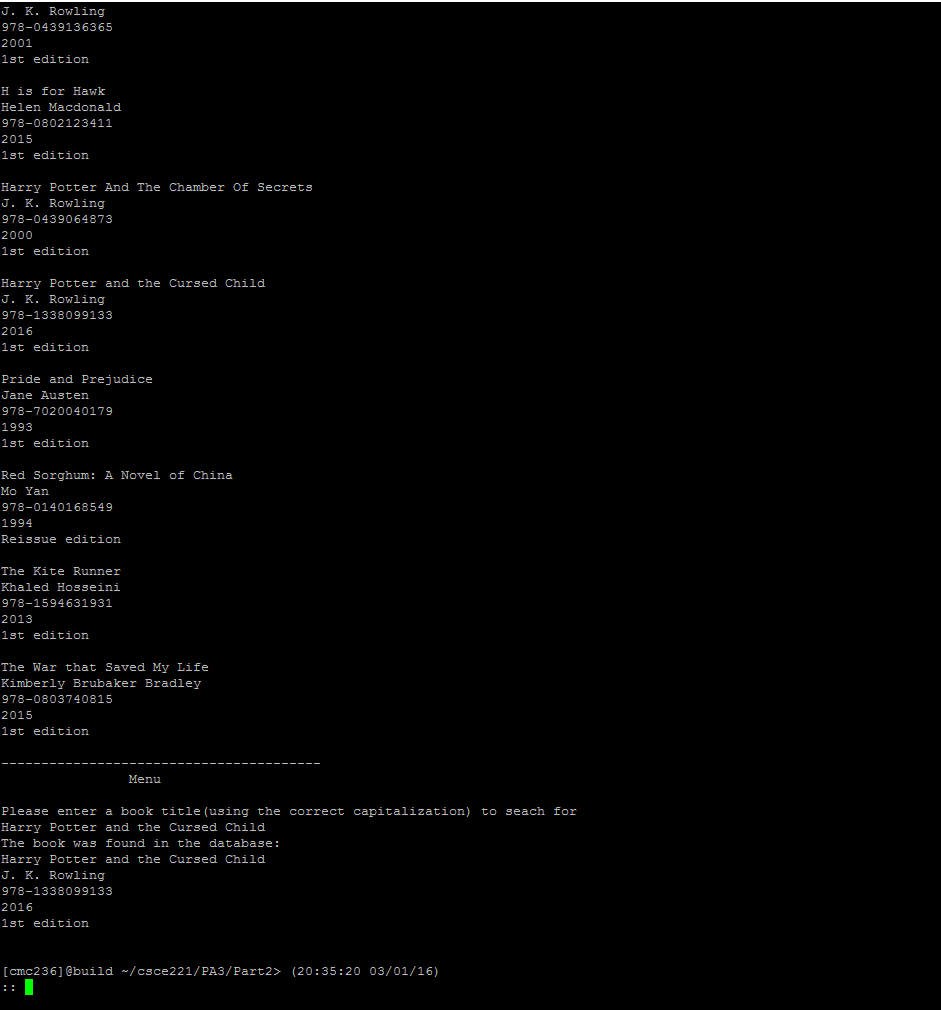
\includegraphics[scale=0.5]{E:/Chris/Pictures/Capture.PNG}


\subsection*{Invalid case:}

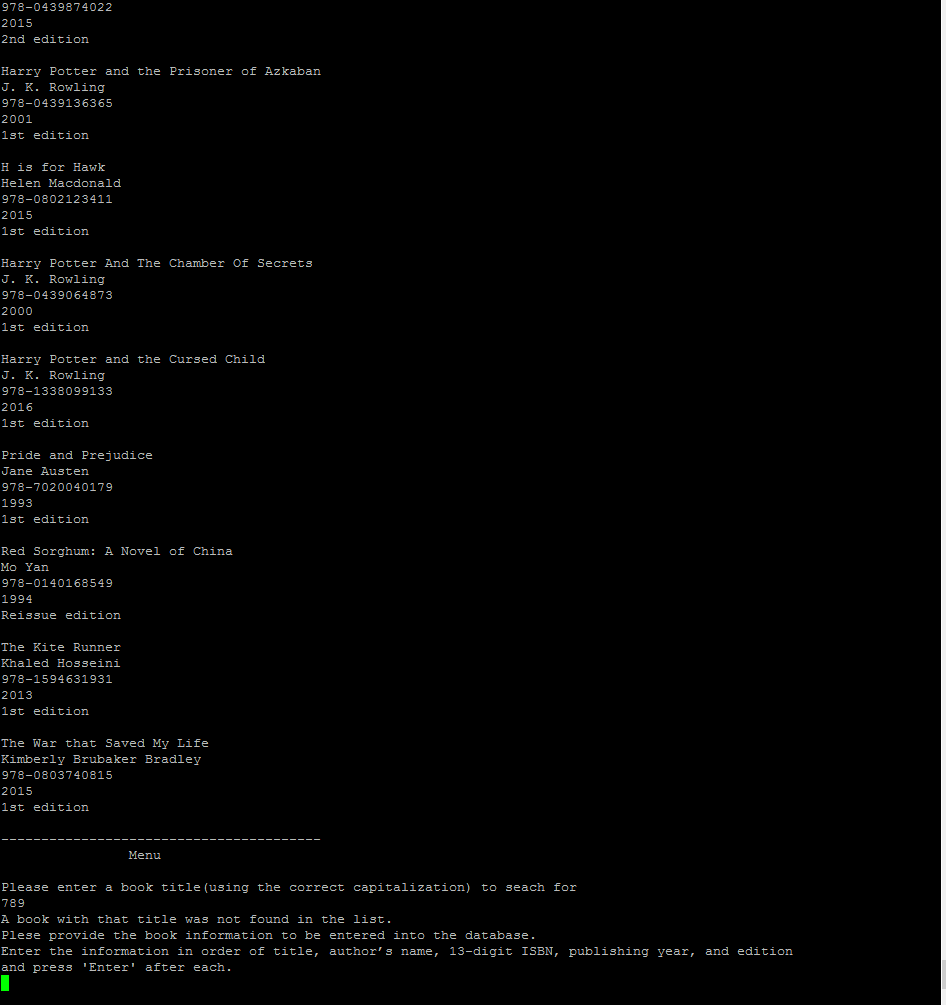
\includegraphics[scale=0.5]{E:/Chris/Pictures/Capture1.PNG}
\end{document}
